\chapter{Koma Higikorreko Aritmetika.}

\section{Sarrera.}

Gaur-egungo konputagailuetan, IEEE-754 estandarraren araberako koma-higikorreko aritmetika erabiltzen da. Koma-higikorreko aritmetikaren gaiak ez dira zenbaki errealak, koma-higikorreko zenbakiak baizik. Zenbaki errealak bit kopuru finituen bidez adierazten dira eta adierazpen finitu honek, biribiltze errorea eragiten du. Zenbakizko integrazio luzeetan  biribiltze errorearen garapenak garrantzia handia du eta errore honen gaineko ahalegin berezia beharrezkoa da.    

\section{Adierazpena.}

\paragraph*{\textbf{Definizioa.}} Koma-higikorreko adierazpen zehatza duen zenbaki errealei koma-higikorreko zenbakiak deritzogu. Koma-higikorreko zenbakien multzoa ${\mathbb{F}}$ izendatuko dugu eta $\phi:\mathbb{F} \rightarrow W$ koma-higikorreko adierazpen funtzioa. 

\begin{equation*}
\mathbb{F}\subset \mathbb{R},
\end{equation*}
\begin{equation}
\mathbb{F}=\{x \in \mathbb{R} \ \mid \ \phi(x) \in W\}.
\end{equation}

\paragraph*{}$\mathbb{F}$ zenbaki multzoa finitua da. Bai zenbaki positiboentzat,bai negatiboentzat, adieraz daitekeen zenbaki handienaren eta txikienaren arteko balio bakanez osatuta dago. Multzoaren kanpoaldean zenbaki hauek guztiak ditugu: batetik overflow tartean $(-\infty,\max_{x \in \mathbb{F_{-}}}|x|)$  eta $(\max_{x \in \mathbb{F_{+}}}|x|,\infty+)$ daudenak; bestetik underflow tartean  $(\min_{x \in \mathbb{F_{-}}}|x|,0)$ eta $(0,\min_{x \in \mathbb{F_{+}}}|x|)$ daudenak. 

\begin{figure}[h]
\centerline{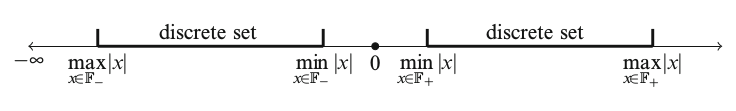
\includegraphics[width=12cm, height=2cm] {KomaHigikorra1}}
\caption{Floating-point number line.}
\label{fig:three}
\end{figure} 

\paragraph*{} IEEE-785 estandarraren arabera, $n$-biteko koma-higikorrezko adierazpenak bi zati ditu,
\begin{enumerate}
\item $m$ bitez osatutako zatia , mantisa deitutakoa eta $M$ zenbaki erreala adierazten duena. Horietako bit bat ($S_M$) zeinua adierazten du. Bestalde $M$ mantisa modu normalizatu honetan emana da, $\pm 1.F$ eta zati erreala ($F$) bakarrik gordetzen da.   
\item Esponentea ($E$), $(n-m)$ bitez adierazitako zenbaki osoa. Zeinuarentzat ez da bit zehatz bat erabiltzen, baizik \it {bias} izeneko balio bat gehituz adierazten dira zenbaki positiboak eta negatiboak.  
\end{enumerate}

\paragraph*{} Eta beraz, oinarri bitarrean koma-higikorreko zenbaki hauek adierazten dira,
\begin{equation*}
M \times b^E, \ b=2.
\end{equation*}

\begin{figure}[h]
\centerline{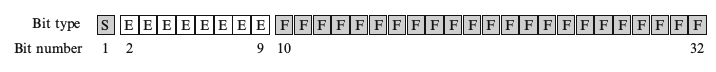
\includegraphics[width=10cm, height=1cm] {KomaHigikorra2}}
\caption[32-biteko koma-higikorra]{\small 32-biteko koma-higikorreko zenbakiaren adierazpena: esponentearentzat 8 bit eta mantisarentzat 24 bit (bit bat zeinuarentzat eta beste 23 bit, $1.F$ eran normalizatutako mantisarentzat) banatuta.}
\label{fig:three}
\end{figure} 

\paragraph*{} 
Bi koma-higikor zenbaki jarraituen arteko diferentzia,
\begin{equation*}
\triangle x=x_1-x_2= 2^{E-m+1}
\end{equation*} 

\paragraph*{}
\it {Machine epsilon} ($\epsilon_M$), $E=0$ deneko koma-higikorrezko bi zenbakien arteko diferentzia bezala definitzen da,
\begin{equation*}
\epsilon_M=2^{-m+1}
\end{equation*} 

\paragraph*{}
Azkenik, \it{roundoff} definituko dugu zenbaki erreal batek koma-higikorrean adierazpenean izan dezakeen errore erlatibo maximoa bezala,
\begin{equation*}
u=\frac{\epsilon_M}{2}=2^{-m}
\end{equation*}  


\paragraph*{}IEEE-785 estandarrean honako formatu bitarrak definitzen dira:

\begin{table} [h!]
\caption{}
\label{tab:1}       % Give a unique label
\begin{tabular}{ |c|c|c|c|c|c|} 
\hline
 Mota      &  Tamaina    & m   & e  & Tartea           &  $u=2^{-m}$           \\ \hline
           &             &     &    &                  &                       \\
% Half      & 16 bit      & 11  & 5  & $2^{\pm 16}$     &  $5 \times 10^{-4}$   \\ 
 Single    & 32 bit      & 24  & 8  & $10^{\pm 38}$    &  $6 \times 10^{-8}$   \\	    
 Double    & 64 bit      & 53  & 11 & $10^{\pm 308}$   &  $1 \times 10^{-16}$   \\
 Quadruple & 128 bit     & 113 & 15 & $10^{\pm 11356}$ &  $1 \times 10^{-35}$   \\
\hline
\end{tabular}
\end{table}

Gaur egungo konputagailuetan, Single eta Double koma-higikorreko aritmetika Hardwarez inplementatuta dago eta oso azkarra da. Single koma-higikorreko aritmetikak Double baino azkarragoa da: batetik garraiatu behar den bit kopuru erdia da eta bestetik, Inteleko txipen \it SSE modulo bereziei esker eragiketa aritmetikoak azkarragoak dira.

2008. urtean, IEEE-785 estandarrak 128 biteko koma-higikorreko aritmetika onartu zuen. Quadruple aritmetika softwarez inplementatuta dago eta horregatik exekuzio motela da, gutxi gorabehera Double aritmetika baino 10 aldiz garestiago. Horretarako hainbat liburutegi daude, guk GCC libquadmath liburutegia aukeratu dugu gure garapeneterako.

Bestalde, badaude doitasun arbitrariotan lan egiteko beste lan-ingurune (Problem Solving Enviroment \cite{Higham2015}) batzuk ere. Doitasun altuetako kalkulu hauekin, soluzio zehatzak lortzen dira eta horrela, algoritmoen testak egiteko bidea ematen dute. Matlab eta Mathematica bezalako softwareetan doitasun handian lan egiteko aukera ematen dute eta beraz, algoritmo berri baten garapenean oso tresna erabilgarriak izan daitezke.

 
\section{Biribiltze errorea.}

Zenbakizko integrazioen errorea, trunkatze eta biribiltze erroreez osatuta dago. Urrats tamaina adina txikia aukeratuz, trunkatze errorea biribiltze errorea baino txikiago izango da eta beraz, zenbakizko integrazioaren errorean biribiltze errorearen eragina nagusituko da. Biribiltze errorea gutxitzea funtsezkoa izango da epe luzeko integrazioetan.     

Bi motako biribiltze errorea dugu, bata adierazpen errorea eta beste eragiketa (aritmetika) errorea.  

\subsection*{Adierazpen errorea.} 

$x \in \mathbb{R}$ eta $fl: \mathbb{R} \rightarrow \mathbb{F}$ 
koma-higikorreko gertuen dagoen zenbakia esleitzen duen funtzioa emanik, errore absolutua,

\begin{equation*}
\triangle x= fl(x)-x= \tilde{x}-x,  
\end{equation*}    
 
eta errore erlatiboa, 
\begin{equation*}
\delta x =\frac{\triangle x}{x} = \frac{\tilde{x}-x}{x}. 
\end{equation*}

Aurreko bi definizioen ondorioz honako formula erabilgarria dugu,
\begin{equation*}
\tilde{x}= x+\triangle x = x(1+\delta x),
\end{equation*}
zeinek IEEE-785 estandarrak $|\delta x|<u$ dela bermatzen duen.

\subsection*{Eragiketen errorea.} 
 
Zenbaki errealen arteko funtsezko eragiketak  $\ast: \mathbb{R}^2\rightarrow \mathbb{R}$, hauek dira
\begin{equation*}
\ast\in \{+,-,x,/ \}.
\end{equation*}

Modu berean, koma-higikorrezko zenbakien arteko funtsezko eragiketak hauek dira $\circledast: \mathbb{F}^2\rightarrow \mathbb{F}$
\begin{equation*}
\circledast\in \{\oplus,\ominus,\otimes,\oslash \}.
\end{equation*}

$\tilde x,\tilde y \in \mathbb{F}$ emanik eta $z= \tilde x \ast \tilde y$ emaitza zehatza bada, $\tilde z= \tilde x \circledast \tilde y$ eragiketaren emaitzaren errore absolutua eta errore erlatiboa definituko ditugu,
\begin{equation*}
\triangle z=\tilde z-z =(\tilde x \circledast \tilde y) -(\tilde x \ast \tilde y)
\end{equation*} 

\begin{equation*}
\delta z=\frac{\triangle z}{z}==\frac{(\tilde x \circledast \tilde y) -(\tilde x \ast \tilde y)}{(\tilde x \ast \tilde y)}
\end{equation*} 

Modu berean honako erlazio dugu,
\begin{equation*}
\tilde z=(\tilde x \circledast \tilde y)=z+\triangle z=z(1+\delta z),  
\end{equation*}
eta IEEE-785 estandarrak \ $|\delta z|<u$ dela bermatzen du.


\paragraph*{\textbf{Adibidea.}}

Errore erlatiboak emaitzaren digitu zuzenak neurtzen du:
\begin{equation*}
\delta z \approx 10^{-k} \Rightarrow \ \approx \ k \ \mbox{digitu hamartar zuzen}.
\end{equation*}  

\subsection*{Ezabapen arazoa.}

Algoritmoen kalkuluetan, doitasuna galera azkarra gerta daiteke. Horren adibidea ezabapen arazoa dugu: oso antzekoak diren bi zenbaki arteko kendura egiten dugunean gerta daitekeena; edo magnitude oso ezberdinak diren bi zenbaki gehitzen ditugunean. 

\paragraph*{\textbf{Adibidea}.}

\begin{lstlisting} [language=Mathematica]
>>  InputForm[N[Pi]]
>> 3.141592653589793

>> y=N[Pi]*10^(-10);
>> InputForm[y]
>> 3.1415926535897934*10^(-10)

>> z=1.+y;
>> InputForm[z]
>> 1.0000000003141594           # 16-digitu hamartar zuzenak.

>> InputForm[z-1.]
>> 3.141593651889707*10^(-10)   # 6-digitu hamartar zuzenak.

\end{lstlisting}
 
\subsection*{Biderketa.}

Orokorrean, $m$ digituzko bi mantisen biderketaren emaitza zehatza adierazteko, $2m$ digituzko mantisa behar dugu ($m$ digituzko galera) \cite{Fukushima2001}. Biderkagaietako bat $2$ren berredura bat bada, orduan biderketa zehatza da baina oro har, $m$ digitu galduko ditugu.  

\paragraph*{} Adibidea.
\begin{equation*}
1,343 \times 2,103 = 2,824229 
\end{equation*} 

\begin{equation*}
1,343 \times 2,103 \approx 2.824
\end{equation*}    


\subsection*{Errore propagazioa.}

Konputazioetan, eragiketa aritmetiko kopuru handia egin behar dugu emaitza lortzeko eta biribiltze errorea metatu daiteke. Batzuetan, eragiketa bakoitzeko biribiltze errorea elkar ezereztatzen da baina kasu txarrenean, biribiltze errorea metatu eta magnitude handikoa izan daiteke.   

\paragraph*{\textbf{Adibidea}.} 
Modu honetako batura batean , non $n>2$ eta $\tilde x_1,\dots,\tilde x_n \in \mathbb{F}$,  ezin daiteke bermatu,  
\begin{equation*}
\bigoplus_{i=1}^{n}(\tilde x_i)=(\sum\limits_{i=1}^{n} \tilde x_i)(1+\delta), \ |\delta|<u.
\end{equation*}

\paragraph*{}Eta $n=3$ deneko adibidean,
\begin{equation*}
((\tilde x_1 \oplus \tilde x_2) \oplus \tilde x_3)  = 
  (\tilde x_1 + \tilde x_2)(1+\delta_1)(1+\delta_2)
  +\tilde x_3 (1+\delta_2), \ \ \delta_1,\delta_2<u.
\end{equation*}

\subsection{Tresnak.}
\subsubsection*{Batura konpensatua.}
   
Batura errekurtsiboetan, biribiltze errorea gutxitzeko metodoa dugu \cite{Higham2002}.
Ideia da, bi zenbakien baturan egindako biribiltze errorearen estimazioa lortu eta estimazio hau hurrengo baturan erabiltzea.

\paragraph*{} Estimazioa nola kalkulatu azaltzeko ikus irudia (Irudia \ref{fig:lau}). Koma-higikorreko bi zenbaki baditugu, $\tilde x,\tilde y \in \mathbb{F}$ non $|\tilde x| \geq |\tilde y|$, eta $\tilde z= \tilde x \oplus \tilde y$ ,

\begin{equation*}
\tilde e= - \bigg(\big(( \tilde x \oplus \tilde y) \ominus \tilde x\big) \ominus \tilde y\bigg) = (\tilde x \ominus \tilde z) \oplus \tilde y
\end{equation*}  

\begin{figure}[h]
\centerline{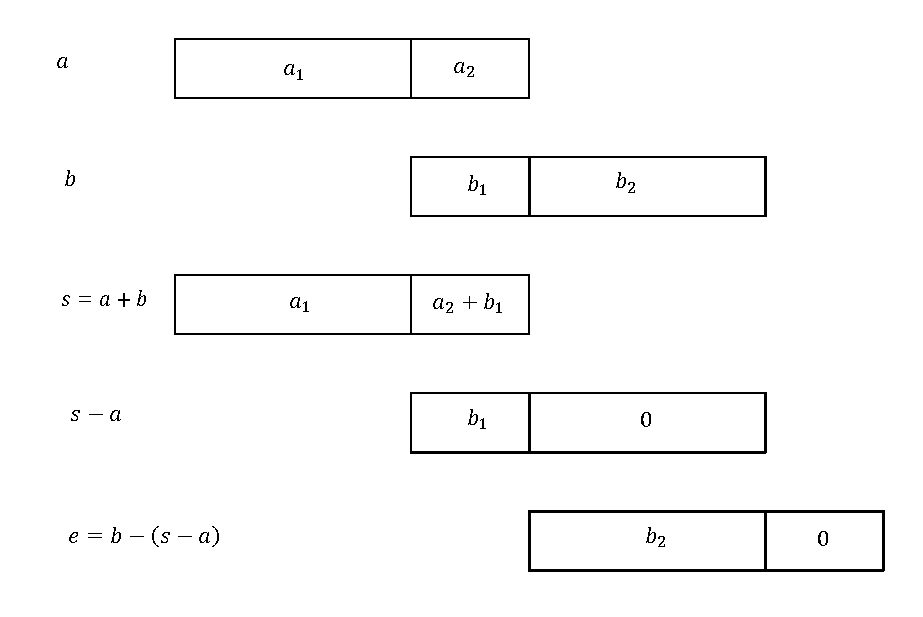
\includegraphics[width=12cm, height=4cm] {Quick2Sum}}
\caption{Biribiltze errorea.}
\label{fig:lau}
\end{figure} 

Lortutako errore estimazioa, koma-higikorreko aritmetikan zehazki benetako biribiltze errorea da,
\begin{equation*}
\tilde x+\tilde y= \tilde z+\tilde e.
\end{equation*}

\paragraph*{} Batura konpensatu algoritmoa biribiltze errore honen estimazioan oinarritzen da. Honako batura  $z=\sum\limits_{i=1}^{n} \tilde x_i$ kalkulatzeko , urrats bakoitzaren amaieran errore estimazioa ($e$) kalkulatuko dugu eta hurrengo urratsean,  batugaiari gehituko diogu ($y=\tilde x_i+e$).

\begin{algorithm}[H]
 \BlankLine
  $z=0; e=0$\;
  \For{$i\leftarrow 1$ \KwTo $endstep$}
  {
   \BlankLine
    $x=z$\;
    $y=\tilde x_i+e$\;
    $z=x+y$\;
    $e=(x-z)+y$\;
   \BlankLine
  }
 \caption{Batura konpensatua.}
\end{algorithm}

\subsubsection*{Biderketaren errore estimazioa.}
Konputagailu berrietan , hardware unitate bereziak bermatzen du biribiltze errore bakarra era honetako eragiketean,

\begin{equation*}
\tilde x \otimes \tilde y \oplus \tilde z= (\tilde x \times \tilde y+ \tilde z) (1+\delta), \ \delta<u.
\end{equation*}

Orduan konputagailuak FMA (fused multiply-add) eragiketak exekutatzen dituela esan ohi da. Hau honela den kasuetan, modu errezan estimatu daiteke biderketa baten biribiltze errorea,


\begin{equation*}
\tilde{z}=\tilde{x}\otimes\tilde{y}, \ \ \tilde{e}=(\tilde{x}\otimes\tilde{y})\ominus \tilde{z}
\end{equation*}


\subsubsection*{Sterbenz Teorema.}
Sterbenz teoremaren arabera \cite{Sterbenz1973}, bi zenbaki elkarrekiko  gertu daudenean,  horien arteko kendura zehatza da.

\begin{equation}
\label{eq:4311}
x,y \in \mathbb{F}, \ \ \frac{y}{2}\leq x \leq 2y \ \ \ \Rightarrow \ \ \ x-y\in \mathbb{F}
\end{equation}




\section{Laburpena.}

Koma-higikorreko aritmetikan sakontzeko honako biografia azpimarratuko dugu, Overton \cite{Overton2001}, Muller  \cite{Muller2009} eta Corless \cite{Corless2013}.

